\chapter{Progetto Interconnect}

Il progetto Interconnect ha l'obiettivo di introdurre concetti per l'interoperabilità e l'integrazione dei dati da diverse fonti, in modo che gli utenti possano fornire i propri servizi e accedere a informazioni pertinenti e correlate in modo più efficiente.


\section{Ontologie Interconnect}
Interconnect non è una singola ontologia, è una famiglia di ontologie che si basano sull'uso di ontologie già esistenti oltre a estendere SAREF e relative estensioni per l'energia.
Nella figura \ref{fig:panoramicaInterconnect} viene raffigurata una panoramica sulle ontologie create all'interno del progetto, mostrando le altre ontologie utilizzate ed estese. In particolare si può notare la famiglia SAREF di ETSI (SAREF e relative estensioni già trattate nel capitolo \ref{cap:panoramicaSaref}).
\begin{figure}[!ht]
    \centering
    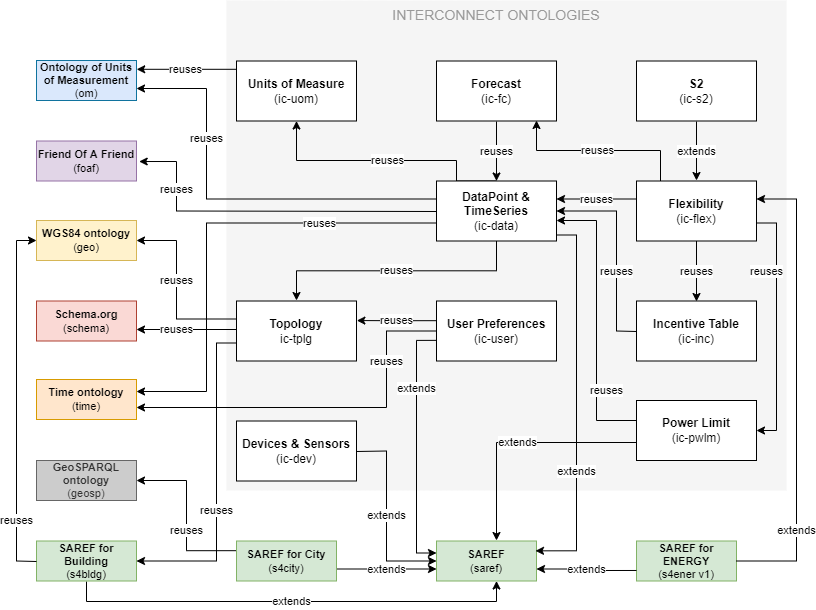
\includegraphics[width=\textwidth]{figures/panoramicaInterconnect.png}
    \caption{Panoramica delle ontologie InterConnect in relazione a SAREF e ad altre ontologie esistenti.}
    \label{fig:panoramicaInterconnect}
\end{figure}

\subsection{Ontologie create nel progetto Interconnect}

\subsection{Ontologie utilizzate}

\section{InterConnect Interoperability Framework}